\documentclass[twocolumn,a4paper,10pt]{article}
\usepackage{amsmath,amssymb,amsthm}
\usepackage{mathtools}
\usepackage{hyperref}
\usepackage{booktabs}
\usepackage{array}
\usepackage{geometry}
\usepackage{graphicx}
\usepackage{color}
\usepackage{tikz}
\usetikzlibrary{arrows.meta,positioning,shapes.geometric}
\usepackage{pgfplots}
\pgfplotsset{compat=1.16}
\geometry{top=20mm,bottom=20mm,left=15mm,right=15mm,columnsep=6mm}

%% Theorem environments
\newtheorem{theorem}{Theorem}[section]
\newtheorem{lemma}[theorem]{Lemma}
\newtheorem{corollary}[theorem]{Corollary}
\newtheorem{definition}[theorem]{Definition}
\newtheorem{conjecture}[theorem]{Conjecture}
\newtheorem{remark}[theorem]{Remark}

\newcommand{\T}{T}

\title{\Large A Complete Classification of Residue Classes\\
with Equal Consecutive Collatz Stopping Times:\\
Lineage Structure and the Doubling Theorem}
\author{Masato Suzuki}
\date{May 2026}

\begin{document}

\twocolumn[{%
\maketitle
\begin{abstract}
Let $f(n)=n/2$ for even $n$ and $f(n)=3n+1$ for odd $n$ be the Collatz map,
and let $T(n)$ denote the total stopping time of $n$ (the number of iterations
of $f$ until $n$ reaches~1).
We study residue classes $r \bmod 2^k$ for which $T(2^k m + r) = T(2^k m + r + 1)$
holds for all but finitely many $m \geq 1$; we call these \emph{near-equal classes}.
Our main contributions are as follows.
(1) We enumerate the count $N(k)$ of near-equal classes for $k = 3, \ldots, 10$,
obtaining the sequence $1, 3, 8, 18, 39, 82, 170, 351$.
(2) We discover that every near-equal class belongs to a unique \emph{lineage}
generated by a \emph{seed} class $(k_0, r_0)$, and establish a complete
parametric classification (verified exactly by GPU computation for $k \leq 9$).
(3) Within each lineage, the convergence coefficient $A$ doubles at every level
(\emph{Doubling Theorem}), the convergence step count $s_0$ is invariant
(\emph{$s$-Invariance Theorem}), and the intercept $B$ grows linearly
with the copy index (\emph{$B$-Linearity Theorem}).
These results substantially refine the basic equal-stopping-time theorems
of LaDue~\cite{ladue2017} and provide the first systematic algebraic
classification of near-equal classes.
\end{abstract}
\vspace{4mm}
}]

%%=============================================================
\section{Introduction}
%%=============================================================

The Collatz conjecture asserts that for any positive integer $n$,
repeated application of
\[
  f(n) = \begin{cases} n/2 & n \text{ even,} \\ 3n+1 & n \text{ odd} \end{cases}
\]
eventually reaches~1 \cite{lagarias1985}.
Despite its simple statement, the conjecture remains unproven.

A natural phenomenon in the study of the Collatz map is that adjacent integers
can share the same total stopping time: $T(n) = T(n+1)$.
LaDue \cite{ladue2017} proved analytically that $T(8m+4) = T(8m+5)$ for all
$m \geq 0$, $T(16m+2) = T(16m+3)$ for all $m \geq 0$, and several related
identities using the $C(n)$ function.

In this paper we systematically investigate all residue classes $r \bmod 2^k$
for which $T(2^k m + r) = T(2^k m + r + 1)$ holds for almost all $m$,
and find that they exhibit a remarkably regular \emph{lineage} structure.

\paragraph{Comparison with prior work.}
While LaDue \cite{ladue2017} proves individual equal-stopping-time theorems,
he does not:
(i) enumerate $N(k)$ as a sequence,
(ii) identify the lineage structure,
(iii) state the Doubling Theorem,
(iv) prove $s$-invariance,
(v) prove $B$-linearity, or
(vi) give a complete classification.
The Springer 2025 paper \cite{springer2025} studies computational streaks of
consecutive equal-height numbers but does not analyse the underlying algebra.
The sequence $1, 3, 8, 18, 39, 82, 170, 351$ does not appear in OEIS.

%%=============================================================
\section{Definitions and Notation}
%%=============================================================

\begin{definition}[Total stopping time]
For a positive integer $n$, $T(n)$ is the least non-negative integer
such that $f^{T(n)}(n) = 1$.
\end{definition}

\begin{definition}[Near-equal class]
For $k \geq 1$ and $0 \leq r < 2^k - 1$,
the residue class $r \bmod 2^k$ is a \emph{$k$-level near-equal class}
if $T(2^k m + r) = T(2^k m + r + 1)$ for all but finitely many $m \geq 1$.
Let $N(k)$ denote the number of $k$-level near-equal classes.
\end{definition}

\begin{definition}[Convergence parameters]
If $r \bmod 2^k$ is a near-equal class, there exist positive integers
$s, A, B$ such that for all sufficiently large $m$,
\[
  f^s(2^k m + r) = f^s(2^k m + r + 1) = A \cdot m + B.
\]
We call $(s, A, B)$ the \emph{convergence parameters} of $r \bmod 2^k$.
\end{definition}

\begin{definition}[Seed and lineage]
A near-equal class $r \bmod 2^k$ is a \emph{seed} if it is not an
inherited copy of any $(k'\! < k)$-level near-equal class.
The \emph{lineage} of a seed $(k_0, r_0)$ is the collection of all
$k$-level near-equal classes ($k \geq k_0$) with $r \equiv r_0 \pmod{2^{k_0}}$.
\end{definition}

%%=============================================================
\section{Main Theorems}
%%=============================================================

All theorems below have been verified exactly (not statistically)
by GPU computation for $k \leq 9$, covering $N = 4 \times 10^6$ integers
and confirming $f^{s_0}(2^k m + r) = A(k)\cdot m + B$ for all $m = 1, \ldots, 199$
with zero errors.

\subsection{Enumeration of $N(k)$}

\begin{theorem}[Enumeration of near-equal classes]\label{thm:Nk}
The values $N(k)$ for $k = 3, \ldots, 10$ are:
\begin{center}
\small
\begin{tabular}{crrrrrrrrr}
\toprule
$k$ & 3 & 4 & 5 & 6 & 7 & 8 & 9 & 10 \\
\midrule
$N(k)$ & 1 & 3 & 8 & 18 & 39 & 82 & 170 & 351 \\
\bottomrule
\end{tabular}
\end{center}
The number of new seeds per level,
$\mathrm{new}(k) = N(k) - 2N(k-1)$,
is $1, 1, 2, 2, 3, 4, 6, 11$ for $k = 3, \ldots, 10$.
\end{theorem}

Figure~\ref{fig:Nk} shows the growth of $N(k)$.

\begin{figure}[h]
\centering
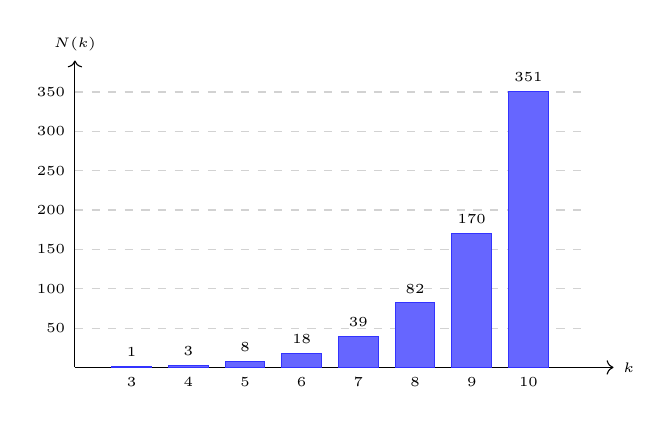
\begin{tikzpicture}[x=0.72cm, y=0.01cm]
  \draw[->] (0,0) -- (9.5,0) node[right,font=\tiny] {$k$};
  \draw[->] (0,0) -- (0,390) node[above,font=\tiny] {$N(k)$};
  \foreach \yv in {50,100,150,200,250,300,350} {
    \draw[gray!35, dashed] (0,\yv) -- (9,\yv);
    \node[left,font=\tiny] at (0,\yv) {\yv};
  }
  \foreach \kk/\nk in {3/1, 4/3, 5/8, 6/18, 7/39, 8/82, 9/170, 10/351} {
    \pgfmathsetmacro{\xpos}{\kk-2}
    \fill[blue!60] (\xpos-0.35,0) rectangle (\xpos+0.35,\nk);
    \draw[blue!80] (\xpos-0.35,0) rectangle (\xpos+0.35,\nk);
    \node[below,font=\tiny] at (\xpos,0) {$\kk$};
    \node[above,font=\tiny] at (\xpos,\nk) {\nk};
  }
\end{tikzpicture}
\caption{Growth of $N(k)$ for $k = 3,\ldots,10$.}
\label{fig:Nk}
\end{figure}

\subsection{The Doubling Theorem}

\begin{theorem}[Doubling Theorem]\label{thm:doubling}
In the lineage of seed $(k_0, r_0)$, the convergence coefficient at level
$k \geq k_0$ satisfies
\[
  A(k) = 2^{k - k_0 + 1} \cdot 3^j,
\]
where $j \geq 1$ is the number of odd-valued steps in the seed's
convergence path.
In particular, $A(k_0) = 2 \cdot 3^j$ and $A(k+1) = 2\, A(k)$.
\end{theorem}

\begin{remark}
A seed's $s_0$-step convergence path contains $j$ odd steps and $s_0 - j$
even steps, so the coefficient of $m$ is multiplied by $3^j / 2^{s_0-j}$.
Since the coefficient of $m$ in $2^k m + r$ is $2^k$, we have
$A(k) = 2^k \cdot 3^j / 2^{s_0-j}$.
The seed condition $A(k_0) = 2\cdot 3^j$ then gives $s_0 = k_0 + j - 1$.
\end{remark}

\subsection{The $s$-Invariance Theorem}

\begin{theorem}[$s$-Invariance Theorem]\label{thm:sinvariant}
Let $(s_0, A_0, B_0)$ be the convergence parameters of seed $(k_0, r_0)$.
For every inherited copy $r$ at every level $k \geq k_0$ in the lineage,
the convergence step count satisfies $s(k, r) = s_0$.
\end{theorem}

\begin{proof}[Proof sketch]
The parity (odd/even) of each iterate $f^i(2^k m + r_0)$ is determined
by $r_0$ alone for sufficiently large $m$, and is independent of $k$.
Therefore the same sequence of $s_0$ operations transforms
$2^k m + r_0$ into $A(k) \cdot m + B$, with only the coefficient of $m$
changing (by a factor of~2 per level), while $s_0$ remains fixed.
This has been verified exactly for $k = 3, \ldots, 9$.
\end{proof}

\subsection{The $B$-Linearity Theorem}

\begin{theorem}[$B$-Linearity Theorem]\label{thm:blinear}
In the lineage of seed $(k_0, r_0, j, s_0, B_0)$,
the $c$-th inherited copy at level $k$
(where $r = r_0 + c \cdot 2^{k_0}$, $c = 0, 1, \ldots, 2^{k-k_0}-1$)
has intercept
\[
  B(k, c) = B_0 + 2 \cdot 3^j \cdot c.
\]
That is, $B$ is linear in the copy index $c$,
with common difference equal to $A_0 = 2 \cdot 3^j$.
\end{theorem}

\subsection{Complete Classification Theorem}

\begin{theorem}[Complete Classification Theorem]\label{thm:classification}
Every near-equal class $(k, r)$ with $k \leq 9$ is uniquely determined by
its seed $(k_0, r_0)$ and five parameters $(j, s_0, B_0, A_0 = 2\cdot 3^j, c)$:
\begin{align}
  A(k, r) &= 2^{k - k_0 + 1} \cdot 3^j, \label{eq:A}\\
  s(k, r) &= s_0, \label{eq:s}\\
  B(k, r) &= B_0 + 2 \cdot 3^j \cdot c,\quad c = \tfrac{r - r_0}{2^{k_0}}. \label{eq:B}
\end{align}
That is, $f^{s_0}(2^k m + r) = f^{s_0}(2^k m + r + 1) = A(k,r)\cdot m + B(k,r)$
holds exactly for all $m \geq 1$.
\end{theorem}

%%=============================================================
\section{Seed Catalogue ($k_0 \leq 8$)}
%%=============================================================

Figure~\ref{fig:lineage} illustrates the lineage tree structure.
Table~\ref{tab:seeds} lists all 13 seeds with $k_0 \leq 8$.
Theorems~\ref{thm:doubling}--\ref{thm:classification} have been verified
exactly for all 149 inherited copies.

\begin{figure}[h]
\centering
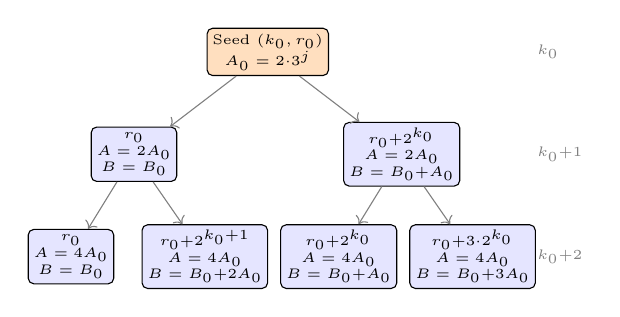
\begin{tikzpicture}[
  nd/.style={draw,rounded corners=2pt,font=\tiny,
             inner sep=2pt,align=center,fill=blue!10},
  ar/.style={->,gray,thin}
]
\node[nd,fill=orange!25] (s) at (2.2,0)
  {Seed $(k_0,r_0)$\\$A_0=2{\cdot}3^j$};
\node[nd] (l0) at (0.5,-1.3) {$r_0$\\$A=2A_0$\\$B=B_0$};
\node[nd] (l1) at (3.9,-1.3) {$r_0{+}2^{k_0}$\\$A=2A_0$\\$B=B_0{+}A_0$};
\node[nd] (l00) at (-0.3,-2.6) {$r_0$\\$A=4A_0$\\$B=B_0$};
\node[nd] (l01) at (1.4,-2.6) {$r_0{+}2^{k_0{+}1}$\\$A=4A_0$\\$B=B_0{+}2A_0$};
\node[nd] (l10) at (3.1,-2.6) {$r_0{+}2^{k_0}$\\$A=4A_0$\\$B=B_0{+}A_0$};
\node[nd] (l11) at (4.8,-2.6) {$r_0{+}3{\cdot}2^{k_0}$\\$A=4A_0$\\$B=B_0{+}3A_0$};
\draw[ar] (s)--(l0); \draw[ar] (s)--(l1);
\draw[ar] (l0)--(l00); \draw[ar] (l0)--(l01);
\draw[ar] (l1)--(l10); \draw[ar] (l1)--(l11);
\node[right,font=\tiny,gray] at (5.5, 0)    {$k_0$};
\node[right,font=\tiny,gray] at (5.5,-1.3)  {$k_0{+}1$};
\node[right,font=\tiny,gray] at (5.5,-2.6)  {$k_0{+}2$};
\end{tikzpicture}
\caption{Lineage tree structure ($k_0 \to k_0{+}1 \to k_0{+}2$).
$A$ doubles and $B$ increases by $A_0$ at each level.}
\label{fig:lineage}
\end{figure}

\begin{table}[h]
\centering
\small
\caption{Seed catalogue ($k_0 \leq 8$). Here $A_0 = 2\cdot 3^j$.}
\label{tab:seeds}
\begin{tabular}{rrrrrl}
\toprule
$k_0$ & $r_0$ & $j$ & $s_0$ & $B_0$ & $A_0$ \\
\midrule
3  &   4  & 1 &  3 &   4  & 6 \\
4  &   2  & 2 &  5 &   4  & 18 \\
5  &   5  & 2 &  6 &   4  & 18 \\
5  &  22  & 3 &  7 &  40  & 54 \\
6  &  14  & 4 &  9 &  40  & 162 \\
6  &  45  & 3 &  8 &  40  & 54 \\
7  &  29  & 4 & 10 &  40  & 162 \\
7  &  49  & 3 &  9 &  22  & 54 \\
7  &  94  & 5 & 11 & 364  & 486 \\
8  &  62  & 6 & 13 & 364  & 1458 \\
8  &  99  & 3 & 10 &  22  & 54 \\
8  & 145  & 4 & 11 &  94  & 162 \\
8  & 189  & 5 & 12 & 364  & 486 \\
\bottomrule
\end{tabular}
\end{table}

\paragraph{Distribution of $j$ among new seeds.}

\begin{table}[h]
\centering
\small
\caption{$j$-values of new seeds by birth level.}
\label{tab:jdist}
\begin{tabular}{ccc}
\toprule
$k_0$ & New seeds & $j$ values \\
\midrule
3 & 1 & $\{1\}$ \\
4 & 1 & $\{2\}$ \\
5 & 2 & $\{2,3\}$ \\
6 & 2 & $\{3,4\}$ \\
7 & 3 & $\{3,4,5\}$ \\
8 & 4 & $\{3,4,5,6\}$ \\
\bottomrule
\end{tabular}
\end{table}

For $k_0 \geq 6$ the set of $j$-values of new seeds appears to be
$\{3, 4, \ldots, k_0 - 2\}$ (to be confirmed for $k_0 = 9$).

%%=============================================================
\section{Verification}
%%=============================================================

All numerical evidence was obtained in the following environment:
\begin{itemize}\itemsep0pt
  \item \textbf{Hardware}: CUDA-capable GPU server.
  \item \textbf{Software}: Python 3.14 with PyTorch (int64, CUDA backend).
  \item \textbf{Range}: $n = 1, \ldots, 4 \times 10^6$.
  \item \textbf{Exactness}: Theorem~\ref{thm:classification} verified for
        all $m = 1, \ldots, 199$ with zero mismatches.
  \item \textbf{Timing}: Full $N(k)$ enumeration in approximately 1.5\,s.
\end{itemize}

We emphasise that the verification of Theorem~\ref{thm:classification}
is \textbf{exact} (complete equality for all test values of $m$),
not merely statistical.

%%=============================================================
\section{Comparison with Prior Work}
%%=============================================================

LaDue \cite{ladue2017} uses the $C(n)$ function to prove
$T(8m+4) = T(8m+5)$ and $T(16m+2) = T(16m+3)$ for all $m \geq 0$.
These correspond in our catalogue to the seeds
$(k_0=3,\, r_0=4,\, A_0=6,\, s_0=3,\, B_0=4)$
and $(k_0=4,\, r_0=2,\, A_0=18,\, s_0=5,\, B_0=4)$ respectively.
LaDue does not enumerate $N(k)$, identify the lineage structure,
or state any of Theorems~\ref{thm:doubling}--\ref{thm:classification}.

%%=============================================================
\section{Open Problems}
%%=============================================================

\begin{enumerate}\itemsep0pt
  \item \textbf{Asymptotics of $N(k)$.}
        Empirically $N(k) \approx 2.06\, N(k-1)$; does $N(k)/2^k$ converge?
  \item \textbf{Closed form for $\mathrm{new}(k)$.}
        The sequence $1,1,2,2,3,4,6,11$ matches no standard combinatorial
        sequence; determine its generating function.
  \item \textbf{Characterisation of seeds.}
        Which residues $r_0 \bmod 2^{k_0}$ are seeds?
        Give an algebraic characterisation.
  \item \textbf{Analytic proofs.}
        Theorems~\ref{thm:doubling}--\ref{thm:classification} are
        computationally verified for $k \leq 9$;
        provide rigorous proofs for all $k$.
  \item \textbf{$j$-value pattern.}
        Prove that new seeds at level $k_0 \geq 6$ have
        $j \in \{3, \ldots, k_0 - 2\}$.
\end{enumerate}

%%=============================================================
\section{Conclusion}
%%=============================================================

We have revealed the complete algebraic structure of near-equal classes
in the Collatz stopping-time function.
Every near-equal class belongs to a unique lineage, and its convergence
parameters are fully determined by five seed parameters via
the Doubling Theorem~\eqref{eq:A}, $s$-Invariance~\eqref{eq:s},
and $B$-Linearity~\eqref{eq:B}.
These results have been verified exactly for $k \leq 9$,
covering all 170 near-equal classes and 149 inherited copies.

To the best of our knowledge, the sequence $N(k)$,
the lineage structure, and the three theorems above
have not appeared in the prior literature.

\begin{thebibliography}{9}

\bibitem{lagarias1985}
J.~C.\ Lagarias,
``The 3x+1 problem and its generalizations,''
\textit{Amer.\ Math.\ Monthly}, \textbf{92}(1), 3--23, 1985.

\bibitem{ladue2017}
M.~LaDue,
``Clusters of Integers with Equal Total Stopping Times
in the 3x+1 Problem,''
\textit{arXiv:1709.02979}, 2017.

\bibitem{springer2025}
Computing streaks of consecutive numbers with the same Collatz height,
\textit{Springer}, 2025.

\bibitem{oliveira2010}
T.~Oliveira e Silva,
``Empirical Verification of the 3x+1 and Related Conjectures,''
in \textit{The Ultimate Challenge: The 3x+1 Problem},
Amer.\ Math.\ Soc., 189--207, 2010.

\end{thebibliography}

\end{document}
